\documentclass[11pt,a4paper]{article}
\usepackage[utf8]{inputenc}
\usepackage[T1]{fontenc}
\usepackage{amsmath}
\usepackage{amssymb}
\usepackage{amsfonts}
\usepackage{graphicx}
\usepackage{hyperref}
\usepackage{geometry}
\usepackage{authblk}
\usepackage{tikz}
\usetikzlibrary{positioning, arrows.meta, shapes.geometric}

\geometry{a4paper, margin=1in}

\title{Mastering Full-Scale Texas Hold'em with Deep Counterfactual Regret Minimization and Transformer Architectures}

% Authorship can be customized as needed
\author[1]{AI Research Group}
\affil[1]{}

\date{}

\begin{document}

\maketitle

\begin{abstract}
Full-scale No-Limit Texas Hold'em (NLHE) presents a monumental challenge for Artificial Intelligence due to its imperfect information nature and vast state space (approximately $10^{160}$ game states). Traditional Counterfactual Regret Minimization (CFR) methods are computationally intractable at this scale. This paper presents a comprehensive framework for developing a state-of-the-art NLHE AI using Deep Counterfactual Regret Minimization (Deep CFR), which leverages deep neural networks for function approximation. We specifically focus on the integration of the Transformer architecture, arguing that its self-attention mechanism is uniquely suited to capturing the complex sequential dynamics of poker. We provide detailed implementation strategies, including structured game state representation, efficient training via weighted sampling (LCFR), the necessity of action translation, and critical pitfalls to avoid for a correct and robust CFR implementation.
\end{abstract}

\section{Introduction}

The pursuit of solving imperfect information games has been a driving force in AI research. No-Limit Texas Hold'em (NLHE), characterized by hidden information and a massive action space, serves as the primary benchmark. Milestones such as Libratus \cite{brown2017superhuman} and Pluribus \cite{brown2019superhuman} demonstrated superhuman performance, relying primarily on variants of CFR applied to heavily abstracted versions of the game.

CFR \cite{zinkevich2007regret} is an iterative algorithm that converges to a Nash equilibrium in zero-sum games by minimizing regret. However, standard tabular CFR requires storing regrets for every information set, which is infeasible in full-scale NLHE.

Deep CFR \cite{brown2018deep} addresses this scalability issue by replacing the tabular storage of regrets with deep neural networks. These networks generalize strategic knowledge across similar information sets, mitigating the need for manual information abstraction.

This paper explores the advancement of Deep CFR by integrating Transformer architectures \cite{vaswani2017attention}. Poker is inherently a sequential game; the strategic implication of a bet depends entirely on the sequence of preceding actions and revealed cards. The Transformer's self-attention mechanism allows the model to dynamically weigh the relevance of different historical events when making a decision, offering a superior approach to function approximation in this domain compared to RNNs or traditional DNNs.

\section{Preliminaries and CFR Foundations}

\subsection{Game Theory Concepts}

We model NLHE as an extensive-form game.
\begin{itemize}
    \item \textbf{Histories (H):} A sequence of actions (by players or chance) starting from the initial state.
    \item \textbf{Information Set (Infoset, I):} A partition of the histories belonging to a player $i$, such that all histories in $I$ are indistinguishable to player $i$. In poker, $I$ is defined by the player's private cards, public cards, and the complete betting history.
    \item \textbf{Strategy Profile ($\sigma$):} A collection of strategies, where $\sigma_i(I)(a)$ is the probability that player $i$ takes action $a$ at infoset $I$.
\end{itemize}

\subsection{Counterfactual Regret Minimization (CFR)}

CFR iteratively updates strategies by minimizing regret. A crucial concept is the \textbf{Counterfactual Value (CFV)}. The CFV for player $i$ at infoset $I$ under strategy profile $\sigma$ is the expected utility, weighted by the probability that opponents and chance allow the state to be reached ($\pi_{-i}^\sigma(I)$). This weighting is critical for focusing optimization on strategically reachable parts of the game tree.

The immediate regret (or advantage) for action $a$ at infoset $I$ in iteration $T$ is:
\begin{equation}
r^T(I, a) = v^\sigma(I, a) - v^\sigma(I)
\end{equation}
Where $v^\sigma(I, a)$ is the CFV of taking action $a$ and then following $\sigma$, and $v^\sigma(I)$ is the average CFV at $I$ under $\sigma$.

The cumulative regret is updated as:
\begin{equation}
R^T(I, a) = R^{T-1}(I, a) + r^T(I, a)
\end{equation}

\textbf{Regret Matching:} The strategy for the next iteration is determined by making actions proportional to their positive cumulative regret:
\begin{equation}
\sigma^{T+1}(I, a) = \frac{R_{+}^{T}(I, a)}{\sum_{a' \in A(I)} R_{+}^{T}(I, a')}
\end{equation}
If the denominator is zero, a uniform random strategy is used.

\section{Deep Counterfactual Regret Minimization (Deep CFR)}

Deep CFR approximates the behavior of CFR in large games by using neural networks to generalize across the vast space of infosets.

\subsection{Architecture Overview}

Deep CFR typically utilizes two main components:

\begin{enumerate}
    \item \textbf{Advantage (Regret) Networks ($V_A$):} Parameterized by $\theta_A$, these networks approximate the immediate regrets (advantages) for actions at a given infoset. $V_A(I; \theta_A) \approx r(I, \cdot)$.
    \item \textbf{Average Strategy:} Traditionally, a separate network ($V_S$) was trained to approximate the average strategy over iterations. However, modern implementations often omit $V_S$ to reduce compound approximation errors. Instead, the average strategy required for evaluation is recovered using Polyak averaging (exponential moving average) of the Advantage Network weights $\theta_A$ across training iterations.
\end{enumerate}

\subsection{Training Procedure: Sampling and Learning}

Deep CFR interleaves data generation (traversal) and network optimization.

\subsubsection{Game Traversal (Data Generation)}

Since the full game tree cannot be traversed, Deep CFR employs Monte Carlo CFR (MCCFR), most commonly \textbf{External Sampling}. External Sampling samples the actions of the opponent(s) and chance events, while iterating over all possible actions for the player being optimized (the "traverser"). This yields lower variance updates.

During traversal, the system queries $V_A$ to determine the current strategy $\sigma^T$, calculates the realized CFVs, computes the realized immediate regrets $r^T(I, a)$, and stores the tuple $(I, r^T(I, a), T)$ in the Advantage Memory Buffer ($M_A$).

\subsubsection{Network Training}

The Advantage Network $V_A$ is trained via supervised learning on the data in $M_A$. The objective is to minimize the difference between the network's predictions and the realized advantages.

\subsection{Stabilization and Optimization}

\begin{itemize}
    \item \textbf{Reservoir Sampling:} Memory buffers ($M_A$) use reservoir sampling to maintain a fixed-size buffer representing a uniform sample of all generated data, crucial for theoretical convergence guarantees.
    \item \textbf{Linear CFR (LCFR):} To accelerate convergence, weighting schemes are employed. LCFR weights the data samples in $M_A$ by the iteration number $T$. This emphasizes recent iterations, reflecting the improving strategy quality.
\end{itemize}

Crucially, when training the neural network, these weights must be incorporated into the loss function. When using LCFR, the Mean Squared Error (MSE) loss for a batch sampled from $M_A$ is formulated as a Weighted MSE:

\begin{equation}
L(\theta_A) = \frac{1}{|B|} \sum_{(I, r, T) \in B} T \cdot (V_A(I|\theta_A) - r)^2
\end{equation}

Where $B$ is the training batch, $\theta_A$ are the network parameters, and $T$ is the iteration number when the sample was generated. Failure to implement this weighted loss correctly will severely hamper convergence.

\section{Applying Transformer Architectures to Poker}

The sequential nature of poker makes it highly suitable for the Transformer architecture. Self-attention allows the model to process the entire game sequence simultaneously and identify relevant relationships between distant events (e.g., relating a river bet back to pre-flop actions).

\subsection{Structured Game State Representation (Input Encoding)}

Encoding the poker infoset requires careful design. A structured approach separates static context from the dynamic history.

\begin{enumerate}
    \item \textbf{Tokenization:} The game history is treated as a sequence of events.
    \begin{itemize}
        \item \textit{Action Tokens:} Represent the type of action (e.g., \texttt{[RAISE]}, \texttt{[CALL]}).
        \item \textit{Card Tokens:} Represent rank and suit (e.g., \texttt{[As]}).
    \end{itemize}

    \item \textbf{Feature Augmentation and Normalization:} Action tokens must be augmented with associated scalar values, such as the bet size. These sizes must be normalized (e.g., as a fraction of the pot, stack depth, or using a logarithmic scale) to generalize across different absolute chip values. These scalar features are typically projected into the embedding space or concatenated with the token embedding.

    \item \textbf{Structured Input Construction:} The input sequence $X$ is constructed by concatenating different segments:
    \begin{itemize}
        \item \textbf{Prefix (Static Context):} Information that remains constant throughout the hand, such as the player's hole cards and their position (e.g., Button).
        \item \textbf{Sequence (Dynamic History):} The sequential history of betting actions and the revelation of community cards (Flop, Turn, River).
    \end{itemize}

    \item \textbf{Positional and Round Encoding:} The order of events is crucial. Positional encodings (sinusoidal or learned) must be added. Furthermore, 'Round-aware' segment embeddings (Pre-flop, Flop, Turn, River) are often added to explicitly delineate the betting rounds.

    \item \textbf{Information Hiding:} The infoset representation must strictly only encode information visible to the acting player. Opponent hole cards must never be included in the input.

\end{enumerate}

\subsection{Network Architecture}

We adapt the standard Transformer Encoder architecture for the Advantage network ($V_A$). An Encoder is appropriate because the entire history leading up to the decision point is available, meaning causal masking is unnecessary.

\begin{itemize}
    \item \textbf{Input Layer:} Processes the structured input embeddings and adds positional/round encodings.
    \item \textbf{Transformer Blocks:} A stack of blocks, each containing Multi-Head Self-Attention and a Feed-Forward Network, utilizing Layer Normalization and residual connections.
    \item \textbf{Output Layer:} The output of the Transformer stack is pooled (e.g., using the embedding of a special \texttt{[CLS]} token added to the prefix, or by applying global average pooling). This aggregated representation is passed through a final linear layer (the "Head") to output the predicted advantages for the discretized set of legal actions.
\end{itemize}

% TikZ Diagram
\begin{figure}[h]
\centering
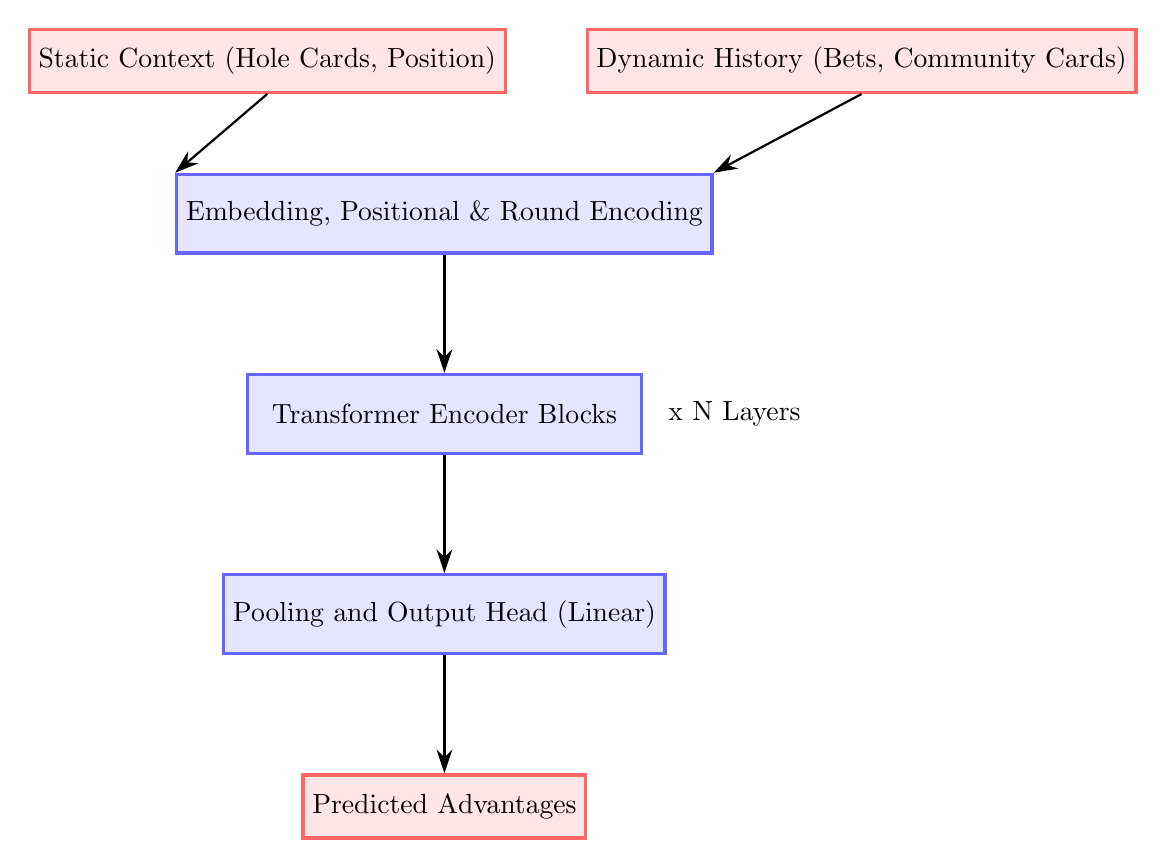
\begin{tikzpicture}[
    node distance=1.5cm,
    block/.style={rectangle, draw=blue!60, fill=blue!10, very thick, minimum height=1cm, minimum width=5cm},
    input/.style={rectangle, draw=red!60, fill=red!10, very thick, minimum height=0.8cm, minimum width=3.5cm},
    arrow/.style={-{Stealth[length=3mm, width=2mm]}, thick}
]

% Nodes
\node (InputPrefix) [input] {Static Context (Hole Cards, Position)};
\node (InputSeq) [input, right=1cm of InputPrefix] {Dynamic History (Bets, Community Cards)};

\node (Embedding) [block, below=1cm of InputPrefix, xshift=2.25cm] {Embedding, Positional \& Round Encoding};

\node (Transformer) [block, below=of Embedding] {Transformer Encoder Blocks};
\node (TransformerLabel) [right=0.2cm of Transformer] {x N Layers};

\node (OutputHead) [block, below=of Transformer] {Pooling and Output Head (Linear)};

\node (Output) [input, below=of OutputHead] {Predicted Advantages};

% Arrows
\draw [arrow] (InputPrefix.south) -- (Embedding.north west);
\draw [arrow] (InputSeq.south) -- (Embedding.north east);
\draw [arrow] (Embedding) -- (Transformer);
\draw [arrow] (Transformer) -- (OutputHead);
\draw [arrow] (OutputHead) -- (Output);

\end{tikzpicture}
\caption{Proposed Transformer Architecture for the Deep CFR Advantage Network utilizing structured inputs (Prefix and Sequence).}
\label{fig:architecture}
\end{figure}

\section{Implementation Details and Challenges}

\subsection{Action Abstraction and Translation}

While Deep CFR reduces the need for \textit{Information Abstraction}, \textit{Action Abstraction} is required for NLHE due to the continuous space of bet sizes. Implementations must restrict allowable bet sizes to a discrete set (e.g., 0.5x pot, 1x pot, 2x pot, All-in).

Crucially, when deployed, an \textbf{Action Translation} mechanism is required. If an opponent makes a bet size not present in the AI's abstraction (an 'off-tree' action), this mechanism maps the action back into the discrete abstraction (e.g., by rounding to the nearest available action). The strategy for the remainder of the hand assumes the translated action occurred.

\subsection{Efficient Distributed Infrastructure}

Training requires a distributed Actor-Learner architecture.
\begin{enumerate}
    \item \textbf{Actors (Data Generators):} Parallel CPU processes execute the MCCFR traversals (External Sampling). They utilize the latest $V_A$ weights and push data into centralized, concurrent Memory Buffers.
    \item \textbf{Learners (Trainers):} GPU/TPU workers continuously sample batches from the Memory Buffers (respecting the LCFR weighting as per Equation 4) to update the Transformer weights.
\end{enumerate}
The efficiency of the game logic and traversal code (often implemented in C++ or Rust) is frequently the system bottleneck.

\subsection{Avoiding Common CFR Errors}

Rigorous validation of the CFR logic is essential, especially when basing implementation on existing codebases which may contain subtle errors.

\begin{itemize}
    \item \textbf{Incorrect Reach Probabilities:} This is the most critical error. CFVs \textit{must} be weighted by the opponent's reach probability ($\pi_{-i}$). Using the player's own reach probability ($\pi_{i}$) breaks the definition of the Counterfactual Value and the theoretical guarantees of CFR.
    \item \textbf{Improper Sampling in MCCFR:} External Sampling must correctly sample chance and opponent actions according to the \textit{current} strategy profile $\sigma^T$. Biased sampling leads to incorrect regret estimates.
    \item \textbf{Errors in Weighted Loss Calculation:} As detailed in Equation 4, the weighting scheme (LCFR) must be correctly applied during the loss calculation, using the iteration number when the data was generated.
    \item \textbf{Information Leakage:} Ensure the infoset representation strictly adheres to the definition and does not include hidden information.
    \item \textbf{Training Stability and Initialization:} Transformers require careful learning rate scheduling (e.g., warm-up and decay with AdamW). Furthermore, it is common practice in Deep CFR to periodically re-initialize the Advantage Network or train from scratch on the entire buffer, rather than continuously fine-tuning, to prevent overfitting to recent samples.
\end{itemize}

Validation should always begin by testing the framework on smaller games (e.g., Kuhn or Leduc poker) and verifying that exploitability converges towards zero.

\section{Evaluation}

Evaluating a poker AI involves assessing how closely it approximates a Nash Equilibrium.

\begin{enumerate}
    \item \textbf{Exploitability (e):} The theoretical measure of performance—how much the AI loses in the worst case against a perfect adversary (Best Response). Calculating this for NLHE is intractable.
    \item \textbf{Approximate Best Response (ABR):} Exploitability is estimated by calculating an approximate best response using localized search (e.g., real-time subgame solving) or Fictitious Play variants against the AI's average strategy.
    \item \textbf{Performance Benchmarking:} Evaluating against known bots by measuring the win rate (in milli-big blinds per game, mbb/g) over a large volume of hands, ensuring statistical significance.
\end{enumerate}

\section{Conclusion}

Deep CFR provides a powerful framework for tackling the immense complexity of No-Limit Texas Hold'em by generalizing strategic knowledge through function approximation. The integration of Transformer architectures represents a significant advancement, as their self-attention mechanism is ideally suited to modeling the sequential dynamics of poker, especially when utilizing structured input representations. Successful implementation requires a meticulous synthesis of game theory (CFR), advanced deep learning techniques (Transformers), high-performance distributed systems, and rigorous attention to the details of weighted sampling, action translation, and regret calculation.

\bibliographystyle{unsrt}
\bibliography{references}

\end{document}